\documentclass[tikz]{standalone}
\begin{document}
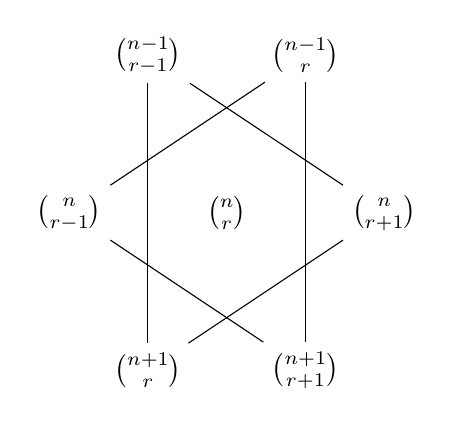
\begin{tikzpicture}
  \node (A) at (1,0) {${{n + 1}\choose{r}}$};
  \node (C) at (4,2) {${{n}\choose{r + 1}}$} edge (A);
  \node (E) at (1,4) {${{n - 1}\choose{r - 1}}$} edge (C)
                                                 edge (A);
  \node (B) at (3,0) {${{n + 1}\choose{r + 1}}$};
  \node (D) at (3,4) {${{n - 1}\choose{r}}$} edge (B);
  \node (F) at (0,2) {${{n}\choose{r - 1}}$} edge (B)
                                             edge (D);
  \node (G) at (2,2) {${n \choose r}$};
\end{tikzpicture}
\end{document}
